\documentclass[shownotes,11pt, aspectratio=169]{beamer}

\usepackage{pgfpages}
% These slides also contain speaker notes. You can print just the slides,
% just the notes, or both, depending on the setting below. Comment out the want
% you want.
\setbeameroption{hide notes} % Only slide
%\setbeameroption{show only notes} % Only notes
%\setbeameroption{show notes on second screen=right} % Both

\usepackage{helvet}
\usepackage[default]{Fira Sans}
\usepackage{array}
\usepackage{caption}
%\usepackage[clean]{svg}
\usepackage{tikz}
\usepackage{verbatim}
\setbeamertemplate{note page}{\pagecolor{yellow!5}\insertnote}
\usetikzlibrary{positioning}
\usetikzlibrary{snakes}
\usetikzlibrary{calc}
\usetikzlibrary{arrows}
\usetikzlibrary{decorations.markings}
\usetikzlibrary{shapes.misc}
\usetikzlibrary{matrix,shapes,arrows,fit,tikzmark}
\usepackage{amsmath}
\usepackage{mathpazo}
\usepackage{hyperref}
\usepackage{lipsum}
\usepackage{multimedia}
\usepackage{graphicx}
\usepackage{multirow}
\usepackage{graphicx}
\usepackage{dcolumn}
\usepackage{bbm}
\usepackage{tfrupee}
\newcolumntype{d}[0]{D{.}{.}{5}}

\usepackage{changepage}
\usepackage{appendixnumberbeamer}
\newcommand{\beginbackup}{
   \newcounter{framenumbervorappendix}
   \setcounter{framenumbervorappendix}{\value{framenumber}}
   \setbeamertemplate{footline}
   {
     \leavevmode%
     \hline
     box{%
       \begin{beamercolorbox}[wd=\paperwidth,ht=2.25ex,dp=1ex,right]{footlinecolor}%
%         \insertframenumber  \hspace*{2ex} 
       \end{beamercolorbox}}%
     \vskip0pt%
   }
 }
\newcommand{\backupend}{
   \addtocounter{framenumbervorappendix}{-\value{framenumber}}
   \addtocounter{framenumber}{\value{framenumbervorappendix}} 
}


\usepackage{graphicx}
\usepackage[space]{grffile}
\usepackage{booktabs}

% These are my colors -- there are many like them, but these ones are mine.
\definecolor{blue}{RGB}{0,114,178}
\definecolor{red}{RGB}{213,94,0}
\definecolor{yellow}{RGB}{240,228,66}
\definecolor{green}{RGB}{0,158,115}

\hypersetup{
  colorlinks=false,
  bookmarks=true,
  linkbordercolor = {white},
  linkcolor = {blue}
}


%% I use a beige off white for my background
\definecolor{MyBackground}{RGB}{255,253,218}

%% Uncomment this if you want to change the background color to something else
\setbeamercolor{background canvas}{bg=MyBackground}

%% Change the bg color to adjust your transition slide background color!
\newenvironment{transitionframe}{
  \setbeamercolor{background canvas}{bg=yellow}
  \begin{frame}}{
    \end{frame}
}

\setbeamercolor{frametitle}{fg=blue}
\setbeamercolor{title}{fg=black}
\setbeamertemplate{footline}[frame number]
\setbeamertemplate{navigation symbols}{} 
\setbeamertemplate{itemize items}{-}
\setbeamercolor{itemize item}{fg=blue}
\setbeamercolor{itemize subitem}{fg=blue}
\setbeamercolor{enumerate item}{fg=blue}
\setbeamercolor{enumerate subitem}{fg=blue}
\setbeamercolor{button}{bg=MyBackground,fg=blue,}



% If you like road maps, rather than having clutter at the top, have a roadmap show up at the end of each section 
% (and after your introduction)
% Uncomment this is if you want the roadmap!
% \AtBeginSection[]
% {
%    \begin{frame}
%        \frametitle{Roadmap of Talk}
%        \tableofcontents[currentsection]
%    \end{frame}
% }
\setbeamercolor{section in toc}{fg=blue}
\setbeamercolor{subsection in toc}{fg=red}
\setbeamersize{text margin left=1em,text margin right=1em} 

\newenvironment{wideitemize}{\itemize\addtolength{\itemsep}{10pt}}{\enditemize}

\title[]{\textcolor{blue}{Macroeconomics: Lecture 4}}
\author[SM]{Sumit Mishra}
\institute[IFMR]{\small{\begin{tabular}{c}
IFMR, Sri City \\
\end{tabular}}}

\date{01 October, 2019}


\begin{document}

%%% TIKZ STUFF
\tikzset{   
        every picture/.style={remember picture,baseline},
        every node/.style={anchor=base,align=center,outer sep=1.5pt},
        every path/.style={thick},
        }
\newcommand\marktopleft[1]{%
    \tikz[overlay,remember picture] 
        \node (marker-#1-a) at (-.3em,.3em) {};%
}
\newcommand\markbottomright[2]{%
    \tikz[overlay,remember picture] 
        \node (marker-#1-b) at (0em,0em) {};%
}
\tikzstyle{every picture}+=[remember picture] 
\tikzstyle{mybox} =[draw=black, very thick, rectangle, inner sep=10pt, inner ysep=20pt]
\tikzstyle{fancytitle} =[draw=black,fill=red, text=white]
%%%% END TIKZ STUFF

% Title Slide
\begin{frame}
\maketitle
%  \centering The views expressed do not necessarily reflect the position of the Federal Reserve Bank of New York or the Federal Reserve System.
\end{frame}

%%SLIDE 1
\begin{frame}
\frametitle{Agenda}
\begin{itemize}
\item Derive the $IS$ relation.
\item Derive the $LM$ relation.
\item $IS-LM$ model.
\item Effect of policy changes on output and interest rates.
\item Material: Blanchard, Chapter 5.
\end{itemize}
\end{frame}

\section{The Goods Market and the $IS$ Relation}
%%%%%%%%%%%%%%%%%%%%%%%%%%%%%%%%%%%%%%%
\begin{frame}{Story Thus Far}
\begin{wideitemize}
\item We know that production = demand for goods. $Y = Z$
\item $Z = C(Y - T) + \bar{I} + G$
\item Interest rate didn't enter our story.
\end{wideitemize}
\end{frame}

%%%%%%%%%%%%%%%%%%%%%%%%%%%%%%%%%%%%%%%
\begin{frame}{Investment, Sales, and the Interest Rate}
Investment is not constant. It depends upon... \pause
\begin{wideitemize}
\item \textbf{The level of sales} \pause $\uparrow$ sales $\Rightarrow$ $\uparrow$ production $\Rightarrow$ $\uparrow$ investments. \pause
\item \textbf{The interest rate} Higher interest rates make investments less attractive. 
\item For now, we assume that there is just one interest rate in our economy.
\item \[ I = I(Y, i) \]
\end{wideitemize}
\end{frame}

%%%%%%%%%%%%%%%%%%%%%%%%%%%%%%%%%%%%%%%
\begin{frame}{Determining Output}
We modify the goods market equilibrium by incorporating the investment relation.
\[ Y = C(Y - T) + I(Y,i) + G \]
For any given interest rate, demand is an increasing function of output.
\begin{wideitemize}
\item $\uparrow$ Output $\Rightarrow$ $\uparrow$ Income $\Rightarrow$ $\uparrow$ Disposable Income $\Rightarrow$ $\uparrow$ Consumption.
\item $\uparrow$ Output $\Rightarrow$ $\uparrow$ Investment.
\end{wideitemize}
\end{frame}

%%%%%%%%%%%%%%%%%%%%%%%%%%%%%%%%%%%%%%%
\begin{frame}{Deriving the $IS$ Curve}
\begin{columns}[T] % align columns
\begin{column}{.44\textwidth}
  \begin{wideitemize}
    \item An increase in interest rate decreases the demand for goods.
    \item This leads to fall in equilibrium level of output.
    \pause
    \item Equilibrium in the goods market: \textcolor{red}{$\uparrow i \Rightarrow \downarrow Y$}
  \end{wideitemize}
\end{column}%
\pause
\hfill%
\begin{column}{.53\textwidth}
  \makebox[\linewidth][c]{
    \resizebox{0.55\linewidth}{!}{
      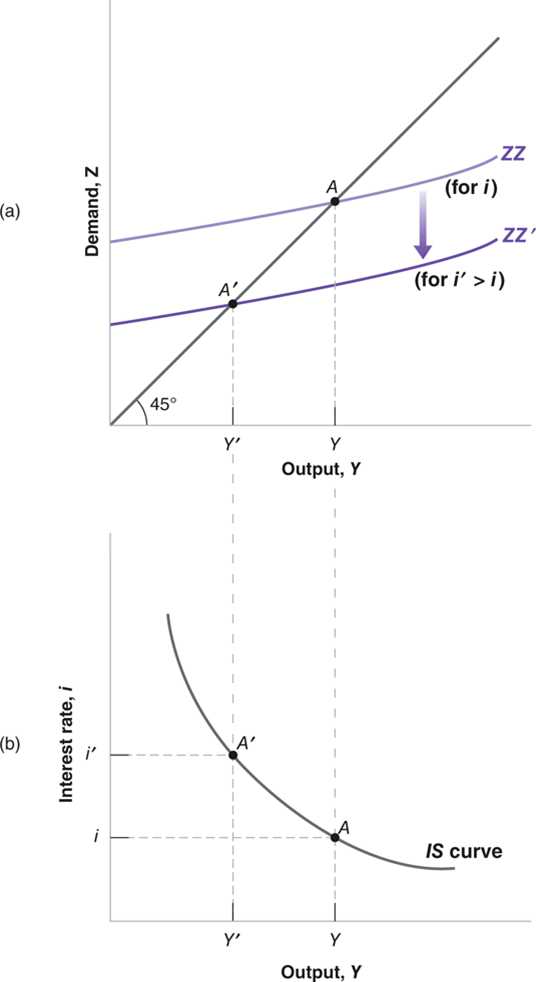
\includegraphics{graphs/L4F2.png}
    }
  }
\end{column}%
\end{columns}
\end{frame}

%%%%%%%%%%%%%%%%%%%%%%%%%%%%%%%%%%%%%%%
\begin{frame}{Shifts in the $IS$ Curve}
\begin{columns}[T] % align columns
\begin{column}{.44\textwidth}
  \begin{wideitemize}
    \item $\uparrow T \Rightarrow \downarrow (Y - T)$.
    \item $\downarrow (Y - T) \Rightarrow \downarrow C$
    \pause
    \item Equilibrium level output would be \textbf{lower}.
    \pause
    \item Changes in factors that \textcolor{red}{decrease} the demand for goods move the $IS$ curve to the left.
  \end{wideitemize}
\end{column}%
\pause
\hfill%
\begin{column}{0.53\textwidth}
  \makebox[\linewidth][c]{
    \resizebox{\linewidth}{!}{
      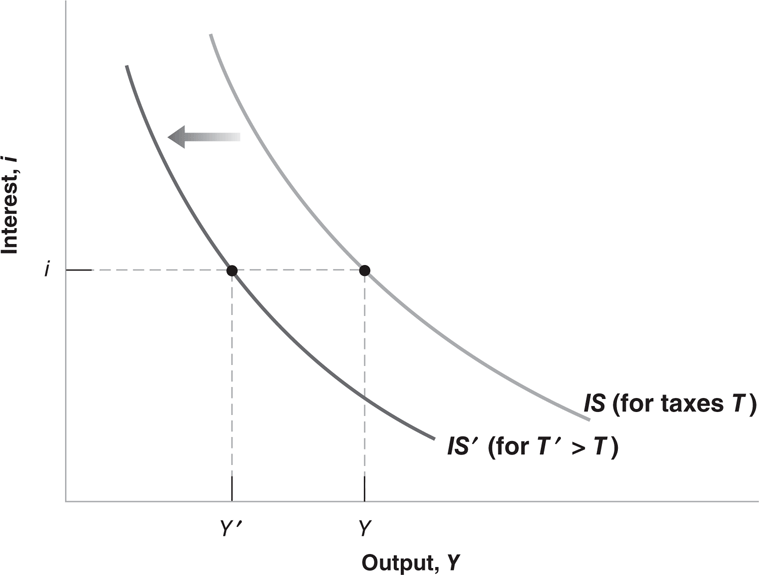
\includegraphics{graphs/L4F3.png}
    }
  }
\end{column}%
\end{columns}
\end{frame}

\section{Financial Market and the $LM$ Relation}
%%%%%%%%%%%%%%%%%%%%%%%%%%%%%%%%%%%%%%%
\begin{frame}{Real Money, Real Income, and the Interest Rate}
\begin{itemize}
\item We modify the money demand equation by introducing price level.
    \[ \frac{M}{P} = YL(i) \]
\item We can now think of equilibrium in terms of \textit{real money demand and supply}.
\item \textbf{Example?}
\pause
\item Think of the cash you would keep to buy two cups of coffee during a class day.
\end{itemize}
\end{frame}


%%%%%%%%%%%%%%%%%%%%%%%%%%%%%%%%%%%%%%%
\begin{frame}{Deriving the $LM$ Curve}
\begin{columns}[T] % align columns
\begin{column}{.44\textwidth}
  \begin{wideitemize}
   \item If interest rate rises, \pause \textcolor{red}{money demand falls}. \pause
   \item What happens to interest rate when income increases? \pause 
   \item $\uparrow Y \Rightarrow \uparrow \text{money demand}$.
   \item The two effects kamikaze each other, and this market is in equilibrium again.
  \end{wideitemize}
\end{column}%
\pause
\hfill%
\begin{column}{.53\textwidth}
  \makebox[\linewidth][c]{
    \resizebox{\linewidth}{!}{
      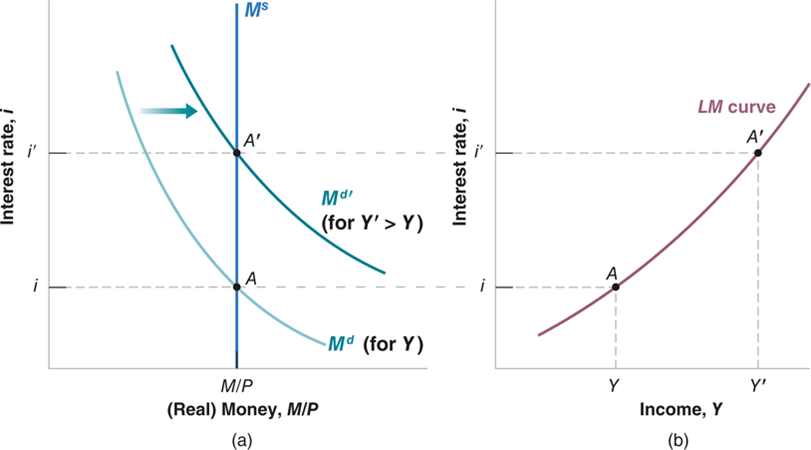
\includegraphics{graphs/L4F4.png}
    }
  }
\end{column}%
\end{columns}
\end{frame}

%%%%%%%%%%%%%%%%%%%%%%%%%%%%%%%%%%%%%%%
\begin{frame}{Shifts: $LM$ Curve}
\begin{columns}[T] % align columns
\begin{column}{.44\textwidth}
  \begin{wideitemize}
   \item Consider a rise in nominal money supply (assume $P$ is fixed).
   \item What happens to real money supply? \pause 
   \item $M/P \rightarrow M^{\prime}/P $ \pause
   \item The $LM$ curve shifts \pause \textcolor{red}{downwards}.
  \end{wideitemize}
\end{column}%
\pause
\hfill%
\begin{column}{.53\textwidth}
  \makebox[\linewidth][c]{
    \resizebox{\linewidth}{!}{
      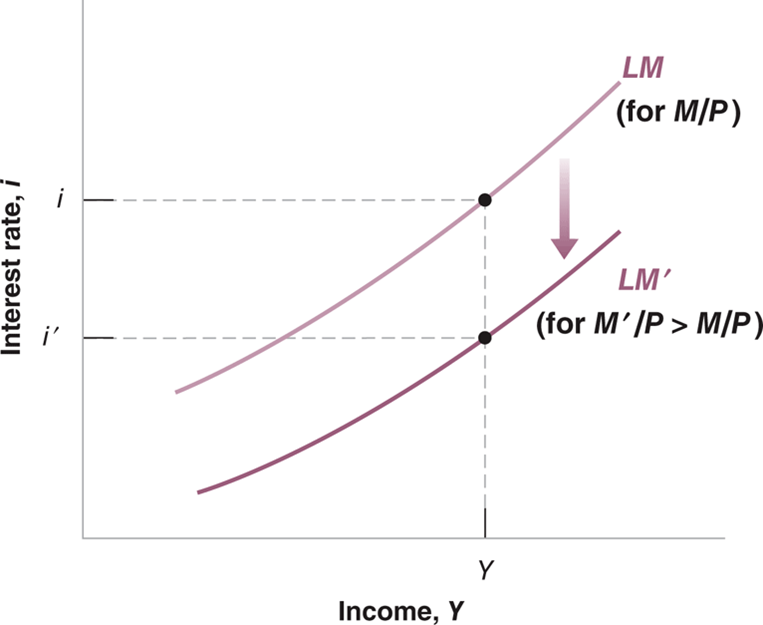
\includegraphics{graphs/L4F5.png}
    }
  }
\end{column}%
\end{columns}
\end{frame}

\section{$IS-LM$ Model}
%%%%%%%%%%%%%%%%%%%%%%%%%%%%%%%%%%%%%%%
\begin{frame}{Putting it all together: $IS-LM$}
\begin{columns}[T] % align columns
\begin{column}{.44\textwidth}
  \begin{wideitemize}
   \item $IS$ relation tells us \pause how \textcolor{red!80}{interest rate affects output}.
   \item $LM$ relation is about \pause how \textcolor{green!80}{output puts pressure on interest rate}. \pause
   \item Mathematically (sorry!):
         \[ IS \text{ equation }:  Y = C(Y - T) + I(Y, i) + G \]
         \[ LM \text{ equation }:  \frac{M}{P} = YL(i) \]
  \end{wideitemize}
\end{column}%
\pause
\hfill%
\begin{column}{.53\textwidth}
  \makebox[\linewidth][c]{
    \resizebox{\linewidth}{!}{
      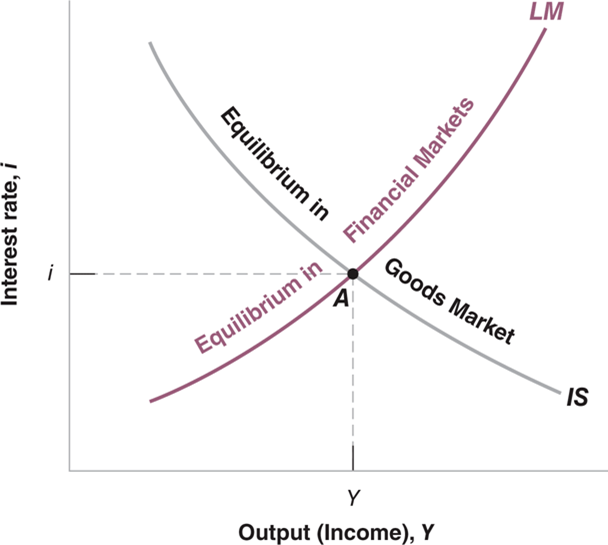
\includegraphics{graphs/L4F6.png}
    }
  }
\end{column}%
\end{columns}
\end{frame}

%%%%%%%%%%%%%%%%%%%%%%%%%%%%%%%%%%%%%%%
\begin{frame}{Fiscal Policy, and the Interest Rate}
\textcolor{red}{Cookbook}
\begin{wideitemize}
\item[1] How does the change affect the goods market and the financial market?
\item[2] Search for the new equilibrium point.
\item[3] Everything needs to be `laypersonized'.
\end{wideitemize}
\end{frame}

%%%%%%%%%%%%%%%%%%%%%%%%%%%%%%%%%%%%%%%
\begin{frame}{Increase in Taxes}
\pause
\begin{wideitemize}
\item What happens to the goods market?
    \begin{itemize}
     \item $\uparrow T \Rightarrow \downarrow Y_D$
     \item $\downarrow Y_D \Rightarrow \downarrow C(Y - T)$. 
     \item $\downarrow C(Y - T) \Rightarrow \downarrow Y$
    \end{itemize}
\pause
\item What happens to the $LM$ curve? \pause \textcolor{red}{Nothing}
\pause
\item \textcolor{red}{Lullaby}: Rising taxes lead to lower disposable consumption $\Rightarrow$ lower consumption $\Rightarrow$ lower income. \pause Declining income $\Rightarrow$ lower money demand $\Rightarrow$ pushes interest rates down.
\pause
\item The net effect would be determined by the size of tax-rise and the quantum of interest rate fall.  
\end{wideitemize}
\end{frame}

%%%%%%%%%%%%%%%%%%%%%%%%%%%%%%%%%%%%%%%
\begin{frame}{Crowding In/Out of Investment}
Because of this rise in taxes, consumption does go down, but what happens to the investments? \pause
\begin{wideitemize}
\item If interest rate is the sole driver of investments, \pause \textcolor{red}{investments should decrease}.
\item If both interest rate and sale determine investments, \pause \textcolor{green}{we need more precise information}.
\pause
\item $\uparrow$ Deficit $\Rightarrow$ $\downarrow$ Investments. We call it \textbf{Crowding Out} of investments.
\item $\uparrow$ Deficit $\Rightarrow$ $\uparrow$ Investments. We call it \textbf{Crowding in} of investments.
\end{wideitemize}
\end{frame}

\begin{frame}
 \makebox[\linewidth][c]{
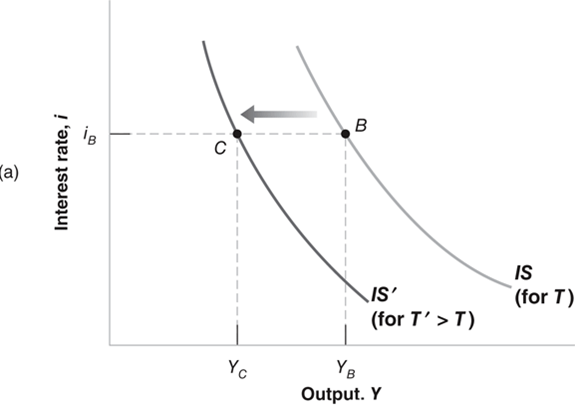
\includegraphics[scale=0.7]{graphs/L4F7.png}}
\end{frame}

\begin{frame}
 \makebox[\linewidth][c]{
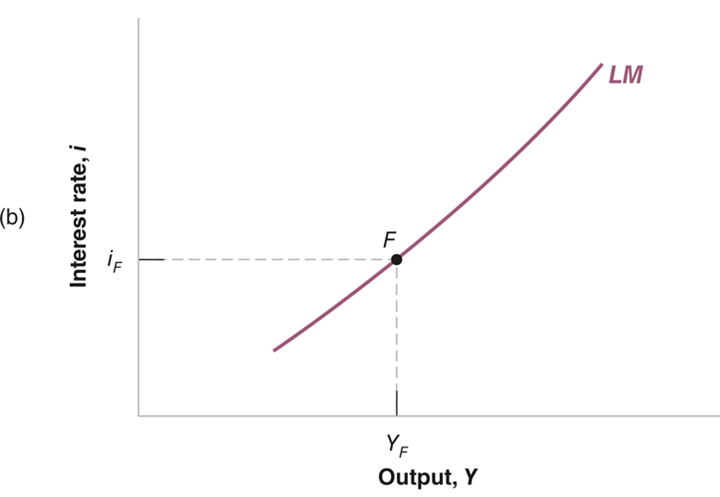
\includegraphics[scale=0.7]{graphs/L4F8.png}}
\end{frame}

\begin{frame}
 \makebox[\linewidth][c]{
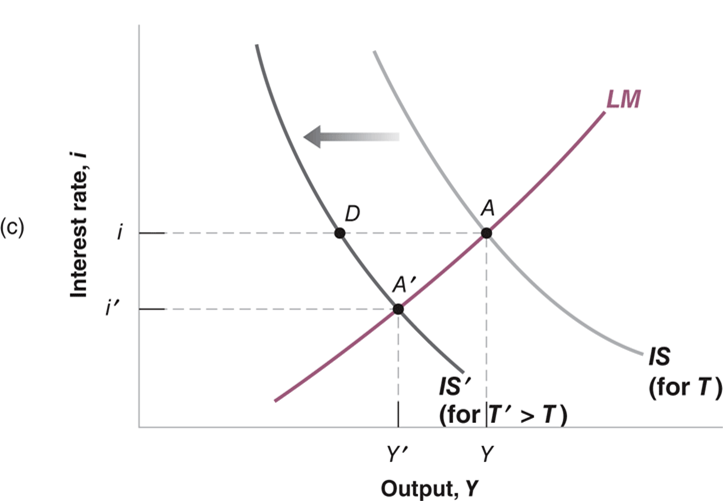
\includegraphics[scale=0.7]{graphs/L4F9.png}}
\end{frame}

%%%%%%%%%%%%%%%%%%%%%%%%%%%%%%%%%%%%%%%
\begin{frame}{Monetary Policy}
Let's discuss the case of monetary expansion or increase in money supply. [Open Market Operation]
\begin{wideitemize}
\item What happens to the financial market?
    \begin{itemize}
    \item If price levels are fixed, $\uparrow M/P$. \pause
    \item $LM$ curve moves downwards. \pause
    \end{itemize}
\item What happens to the goods market? \pause \textcolor{red}{Nothing}  \pause
\item Monetary expansion $\Rightarrow$ $\downarrow i$ and $\uparrow Y$.
\item \textcolor{red}{Lullaby}: Increase in money supply $\Rightarrow$ lower interest rate $\Rightarrow$ increase in investment $\Rightarrow$ higher output and demand. 
\end{wideitemize}
\end{frame}

%%%%%%%%%%%%%%%%%%%%%%%%%%%%%%%%%%%%%%%
\begin{frame}
\makebox[\linewidth][c]{
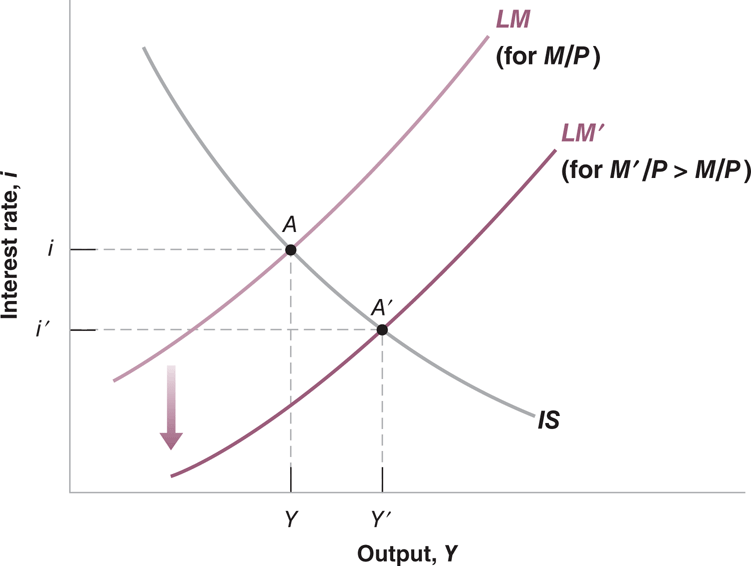
\includegraphics[scale=0.7]{graphs/L4F10.png}}
\end{frame}


%%%%%%%%%%%%%%%%%%%%%%%%%%%%%%%%%%%%%%%
\begin{frame}{The Greek Soup}
What happens when governments try to rescue economy by fiscal contraction?
\begin{itemize}
\item Debts become too large. What's the option? You either reduce expenditure or raise tax rates.
\pause
\item From the theory, we know that increasing tax-rates leads to a fall in output.
\item Therefore, \textit{government reduces not only what it needs to pay, but also the amount that it was going to use to pay those debts.}
\pause
\item Austerity was offered as a panacea for Greek crisis. It didn't work.
\pause
\item What was the other problem? \pause (Hint: Monetary policy)
\end{itemize}
\end{frame}

%%%%%%%%%%%%%%%%%%%%%%%%%%%%%%%%%%%%%%%
\begin{frame}{The Effects of Fiscal and Monetary Policy: Cheatsheet}
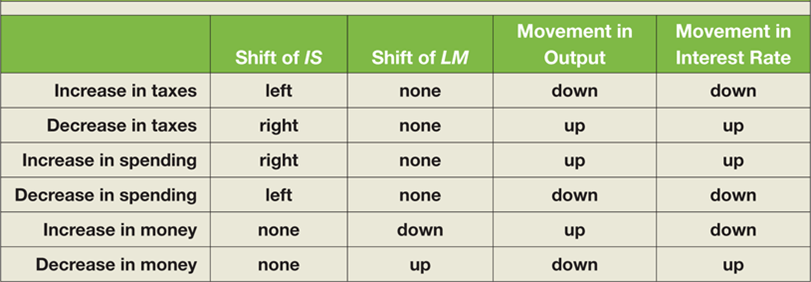
\includegraphics[scale=0.65]{graphs/L4F11.png}
\end{frame}

%%%%%%%%%%%%%%%%%%%%%%%%%%%%%%%%%%%%%%%
\begin{frame}{Using a Policy Mix}
Tackling Recession of 2001 (the US): a combination of monetary expansion and fiscal expansion (expenditure + lower tax rates).
\begin{itemize}
\item 2001: Steep fall in investment demand $\Rightarrow$ $IS$ curve shifts to the left. \pause
\item Response 1: $\uparrow$ Money supply $\Rightarrow$ $LM$ curve shifts downwards. \pause
\item Response 2: $\downarrow$ tax rates \& $\uparrow$ expenditure $\Rightarrow$ $IS$ curve shifts to the right.
pause
\item Because of the two sets of policy decisions, economy could be rescued. \pause
\item What's the problem with this story? \pause (Hint: \textbf{Budget Deficits})
\item Why was the same diagnosis not administered in 2009? 
\end{itemize}
\end{frame}

\end{document}